\documentclass[a4paper, 12pt]{article}

\usepackage{graphicx}
\usepackage{xcolor}
\usepackage{mdframed}
\usepackage { amsmath , amssymb , amsthm }
\usepackage[T2A]{fontenc}
\usepackage[utf8]{inputenc}
\usepackage[english,russian]{babel}

\graphicspath{{img/}}
\DeclareGraphicsExtensions{.pdf,.png,.jpg}


\title{Информатика}
\author{Шмаков И. А.}
\date{\today}

\begin{document}
\sffamily
\maketitle
\section*{№18}
\section*{Лекция 1}
\textbf{Информатика} -- это наука изучающая информационные аспекты процессов и системные аспекты информационных процессов.\\
Термин впрвые появился в 1957 году благодаря Карлу Штейнбуху. В 1962 Дрейфусом во Франции. Харкувич в 1962 в СССР.\\
\textbf{Информация} -- свединия или объект о чем-то
\textbf{Объем данных} -- кол-во байт, необходимых для их хранения в памяти электронного носителя. Бит -- базовая единица измерения кол-ва информации.\\
\textbf{Машинное слово} -- машино-зависящее и платформо-зависящее величина, измеряющаяся в битах или байтах.
\\ Перевод из одной системы счисления в другую:\\
$ 10_{10} \to N_{2} $, делим число на 2 и ее остаток пока не получим 1 и дальше делить не можем и записываем в обратном порядке остатки.\\
Двоичное представление:\\
10:ABCD\\
0:0000\\
1:0001\\
2:0010\\
  ...\\
8:1000\\
\underline{9:1001}\\
10:1010\\
11:1011\\
12:1100\\
13:1101\\
14:1110\\
15:1111\\

Для возвращения в 10ную систему счисления нужно возвести в степень($   1001111_2 = 1\cdot2^6 +1\cdot2^3+1\cdot2^2+1\cdot2^1+1\cdot2^0 = 79_{10}$)




\section*{Лекция 2 -- Информация, кодирование информации, код Шенона и различные кодировки}

\textbf{Данные} -- подающееся многократной интерпретации, предвтавление инфомрации в формализованном виде, пригодном для передачи, связи или обработки.\\

\textbf{Свойства:}\\
1. Объективность\\
2. Достоверность\\
3. Полнота -- минимальный набор, достаточный для принятия решений\\
4. Адекватность \\
5. Доступность\\
6. Актуальность(только вовремя полученная информация является полезной)\\
7. Ценность\\
8. Понятность(ясность)\\
9. Точность\\
10. Атрибутивные св.\\
11. Динамические св.\\
12. Практические св.\\


\textbf{Теория информации} -- раздел прикладной математики, относящиийся к измерению кол-ва информации, ее свойств и устанавливающий предельные соотношения для систем передачи данных.\\
\begin{mdframed}[backgroundcolor=blue!20] 
       
  
\textbf{Схема передачи информации}

Источник информации $\to$ кодер инсточника $\to$ кодер канала $\to$ модулятор $\to$ среда распространения $\to$ демодулятор $\to$ декодер канала $\to$ декодер источниа $\to$ получатель информации
\end{mdframed}

\textbf{Передача информации} -- это заблагавременно организованное техническое мероприятие, результатом которого становится воспроизведение информации, имеющейся в одном месте,в другое место.\\

Мнформационная энтропя -- мера неопределенности или непредсказуемости некоторой системы, в часности неопределенность появления какого-либо символа первичного алфавита.\\
Энтропия -- это количество информации, приходящейся на одно элементароное сообщение источника, вырабатывающейго ...\\

\begin{mdframed}[backgroundcolor=blue!20] 
       Формула Хартли:\\
       \[l = \log_2 (N) = n \log_2 (m)\]
       N - кол-во возможной информации\\
       m - кол-во букв в алфавите\\
       n - кол-во букв в сообщении\\
       $ l $ - кол-во информации в битах\\
       это верно при равновероятном появлении символа\\
    \end{mdframed}



\begin{mdframed}[backgroundcolor=blue!20] 
       Информационная двоичная энтропия для независимых случайных событий:\\
       \[
       	H(x) = -K\sum_{i=1}^n p(i) \log_2 p(i)
       \]
    \end{mdframed}


\section*{Лекция 3. Кодирование данных}

Прямой код -- способ представления двоичных чисел с фиксированной \\

Сумматор -- устройство преобразующее информационные сигналы в сигнал, эквивалентный сумме этих сигналов, устройство производящее операцию сложения.\\
1938 году в "Bell laboratories" создали первый электронныйы двоичный сумматор.\\

Двоичный сумматор может быть описан с помощью:\\
-- таблицы истиности\\
-- в виде формулы\\
-- в виде логической схемы\\

Обратный код -- метод вычислительной математики, позволяющий вычесть одно число из другого используя только операцию сложения над натуральными числами. Обратный код положительного числа совпадает с Прямым кодом.\\

Дополнительный код -- он позволяет заменить операцую вычитания на операцию сложения и сделать операции сложения и вычитания одинаковыми для знаковыз и безнаковых чисел.\\

Форма представления чисел с плавующей точкой состоит с помощью мантисы и показателя степени.\\

Машинный эпсилон -- наименьшее положительное число, такое что неравное 1.\\

Кодирование графических данных:\\
1)Растровое -- сетка из пикселей\\
2)Векторное -- представление объектов с помощью примитивов(точки, линии, спрайты и т.д.)\\
3)Фрактальная --  состоит из фракталов, объектов,отдельные элементы которого наследуют свойства родительской структуры.\\




\section*{Лекция 4. Кодирование звуковой информации}

В основе кодирования звука в пк лежит процесс преобразования колебаний воздуха в колебания электрического тока и последующия дискретизация\\

Аналоговый сигнал -- это сигнал данных у которого каждый из параметров описывается функцией времени и непосредственно множеством возможных значений\\

Дискритизация -- представление непрерывной функции в дискретной совокупности ее значений\\

Частота выборки(дискретизации) -- обратная величина дескритизации\\

Цифровой звук -- результат преобразования аналогового сигнала звукового диапазона в цифровой аудиоформат\\

Цифровая звукозапись -- технология преобразования аналогово звука в цифровой\\

\begin{mdframed}[backgroundcolor=blue!20] 
       Теорема Котельникова:\\
       Фундаментальное утверждение в области цифровой обработки сигналов связывающий непрерывные и дискретные сигналы и гласящее что любую функцию состоящюю из частот от 0 до f1 можно передавать с любой точностью при помощи чисел следующих друг за другом.
    \end{mdframed}
Виды звукозаписи:\\
1)Магнитная \\
2)Магнитострочная\\
3)Лазерная\\
4)Оптическая\\
5)На электронные носители\\

Виды сжатия:\\
-- без потери данных\\
-- с потерей данных\\

Аудиоредактор(волновой) -- для редактирования звуковой информации в цифровом представлении.\\

Цифровая звуковая рабочая станция -- система, предназначенная для записи хранения и редактирования востпроизведения аудио файлов.\\

Форматы без сжатия -- wav,raw\\\
Форматы с сжатием без потерь-- flac,apple lossless\\
Форматы с потерями -- mp2,mp3,wma\\

\begin{mdframed}[backgroundcolor=blue!20] 
       Формула для нахождения звуковой информации
       \[
         N = 2^i
       \]
       N -- кол-во уровней сигнала\\
       i -- глубина звука\\

       Объем звукового файла
       \[
         V_{audio} = o*D*T*i
       \]

    \end{mdframed}
    
Видео -- технология формирования записи,обработки и воспроизведения\\

Видеозапись -- технология записи визуальной информации\\

Цифровое видео -- совокупность технологий для взаимодействия с видео и т.д.\\

Стандарты передачи видео -- NTSC,SECAM,PAL\\

VGA - 640 - 480\\
PAL - 
HD - 1366 - 768\\
FullHD - 1920 - 1080\\
...\\

Кадровая частота -- кол-во сменяемых кадров за единицу времени\\

Разрешающая способность -- способность устройства передавать мелкие детали изображения\\

Стандарт разложения -- определяющая кол-во строк изображения,частоту смены кодров и режим развертки\\

Битрейт -- кол-во битов в единицу времени\\
Качество видео -- характеристика обработанного видео по сравнению с оригиналом\\
Цветовая субдискретизация -- кодирование изображений со снижением цветового разрешения\\

\begin{mdframed}[backgroundcolor=blue!20] 
      Видео дорожка:
       \[
         V_{image} = resolution * v * T * i
       \]

       Размер видео файла:
       \[
         V_{video} = V_{image} + V_{audio}
       \]
    \end{mdframed}

\newpage
\section*{Лекция 5. Алгоритмы сжатия данных}

Сжатие данных -- алгоритмическое преобразованние даных для уменьшения размера\\

Сжатия информации -- процесс преобразования информации хранящейся в файле к виду при котором уменьшается избыточность в ее представлении и соответсвенно треьуется меньший объем памяти для хранения\\

\begin{mdframed}[backgroundcolor=blue!20] 
       Степень сжатия:
       \[
         K_{C} = \frac{V_C}{V_Q} 100 \%
       \]
    \end{mdframed}
    

Метаданные -- информация о другой информации\\

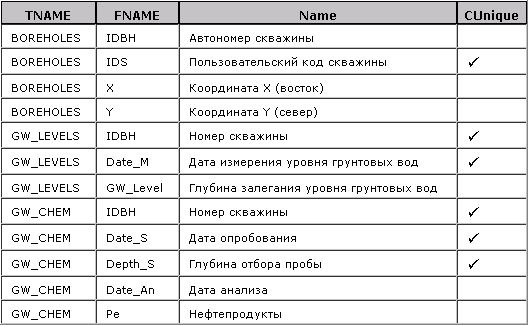
\includegraphics{51}\\

Классификация метаданных:\\
1) по содержание\\
2) по отношению к ресурсу в целом\\
3) по возможности логического вывода\\


\subsection*{RLE алгоритм(кодирование повторово)}
--  алгоритм сжатия данных, заменяющий повторяющиеся символы (серии) на один символ и число его повторов. Серией называется последовательность, состоящая из нескольких одинаковых символов. При кодировании (упаковке, сжатии) строка одинаковых символов, составляющих серию, заменяется строкой, содержащей сам повторяющийся символ и количество его повторов. 

\subsection*{Алгоритм Шенона-Фано}
(\\
1)Символы первичного алфавита m1 выписывают по убыванию вероятностей.\\
2)Символы полученного алфавита делят на две части, суммарные вероятности символов которых максимально близки друг другу.\\
3)В префиксном коде для первой части алфавита присваивается двоичная цифра «0», второй части — «1».\\
4)Полученные части рекурсивно делятся и их частям назначаются соответствующие двоичные цифры в префиксном коде.\\
)\\

Пример кодового дерева\\
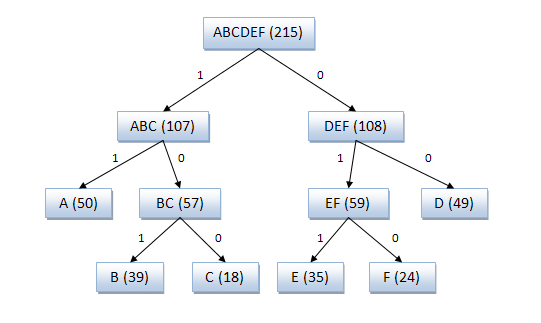
\includegraphics{img/52.PNG}\\

\subsection*{Алгоритм Хаффмана} — жадный алгоритм оптимального префиксного кодирования алфавита с минимальной избыточностью. Был разработан в 1952 году аспирантом Массачусетского технологического института Дэвидом Хаффманом при написании им курсовой работы. В настоящее время используется во многих программах сжатия данных.\\

Этот метод кодирования состоит из двух основных этапов:\\
    Построение оптимального кодового дерева.\\
    Построение отображения код-символ на основе построенного дерева.\\

Классический алгоритм Хаффмана на входе получает таблицу частот встречаемости символов в сообщении. Далее на основании этой таблицы строится дерево кодирования Хаффмана (Н-дерево).\\

    1. Символы входного алфавита образуют список свободных узлов. Каждый лист имеет вес, который может быть равен либо вероятности, либо количеству вхождений символа в сжимаемое сообщение.\\
    2. Выбираются два свободных узла дерева с наименьшими весами.\\
    3. Создается их родитель с весом, равным их суммарному весу.\\
    4. Родитель добавляется в список свободных узлов, а два его потомка удаляются из этого списка.\\
    5. Одной дуге, выходящей из родителя, ставится в соответствие бит 1, другой — бит 0. Битовые значения ветвей, исходящих от корня, не зависят от весов потомков.\\
    6. Шаги, начиная со второго, повторяются до тех пор, пока в списке свободных узлов не останется только один свободный узел. Он и будет считаться корнем дерева.\\


\subsection*{LZ77 и LZ78}
 — алгоритмы сжатия без потерь, опубликованные Абрахамом Лемпелем и Якобом Зивом в 1977 и 1978 годах соответственно. Эти алгоритмы стали основой других алгоритмов семьи LZ*: LZW, LZSS, LZMA и другие. Оба приведенных алгоритма используют словарный подход.\\

\subsection*{Алгоритм Лемпеля — Зива — Велча}
-- это универсальный алгоритм сжатия данных без потерь, созданный Авраамом Лемпелем, Яаковом Зивом и Терри Велчем. Он был опубликован Велчем в 1984 году в качестве улучшенной реализации алгоритма LZ78, опубликованного Лемпелем и Зивом в 1978 году. Алгоритм разработан так, чтобы его было достаточно просто реализовать как программно, так и аппаратно\\

 Более формально данный алгоритм можно описать следующей последовательностью шагов:\\
    1. Инициализация словаря всеми возможными односимвольными фразами. Инициализация входной фразы W первым символом сообщения.\\
    2. Если КОНЕЦ СООБЩЕНИЯ, то выдать код для W и завершить алгоритм.\\
    3. Считать очередной символ K из кодируемого сообщения.\\
    4. Если фраза WK уже есть в словаре, то присвоить входной фразе W значение WK и перейти к Шагу 2.\\
    5. Иначе выдать код W, добавить WK в словарь, присвоить входной фразе W значение K и перейти к Шагу 2.\\


\end{document}